
%(BEGIN_QUESTION)
% Copyright 2011, Tony R. Kuphaldt, released under the Creative Commons Attribution License (v 1.0)
% This means you may do almost anything with this work of mine, so long as you give me proper credit

Suppose you need to ``fool'' this PLC into ``thinking'' that there is a low-pressure condition (less than 24 PSI) when in fact there is not:

$$\includegraphics[width=15.5cm]{i03570x01.eps}$$

Explain how you could do that, without access to a PC to force bits inside the PLC's memory.  Be specific in your answer, sketching the solution on the diagram if desired.

\underbar{file i03570}
%(END_QUESTION)





%(BEGIN_ANSWER)

Jumper from {\tt L1} to terminal {\tt IN2} to force power to that channel.

%(END_ANSWER)





%(BEGIN_NOTES)

{\bf This question is intended for exams only and not worksheets!}.

%(END_NOTES)

